\documentclass{article}

%%%%%%%%%%%%%%%%%%%%%%%%%
% Packages & Macros
%%%%%%%%%%%%%%%%%%%%%%%%%

% For including graphics
\usepackage{graphicx}

% For title page
\usepackage{datetime}
\newdateformat{monthyeardate}{\monthname[\THEMONTH] \THEYEAR}

% For supporting linking
\usepackage{hyperref}
\hypersetup{colorlinks,urlcolor=blue,linkcolor=blue}


%%%%%%%%%%%%%%%%%%%%%%%%%
% Tool-Specific Macros
%%%%%%%%%%%%%%%%%%%%%%%%%
\usepackage{xspace}

\newcommand{\args}[1] {\textit{#1}}
\newcommand{\cmd}[1] {\texttt{#1}}     % Use for command window commands, e.g., \cmd{svn up}
\newcommand{\block}[1] {\textsf{#1}}   % Use for Simulink block names, e.g., \cmd{Subsystem1}
\newcommand{\signal}[1] {\textsf{#1}}   % Use for Simulink block names, e.g., \cmd{Subsystem1}
\newcommand{\ring}[1] {\textsf{#1}} 	 % Use for files names and paths
\newcommand{\keyword}[1] {\texttt{#1}} % Use for keywords of programming languages, e.g., \keyword{while}
\newcommand{\file}[1] {\texttt{#1}} 	 % Use for files names and paths
\newcommand{\param}[1] {\textit{#1}}   % Use for block parameter names, e.g., \param{BlockType}

% Matlab Products
\newcommand{\matlab}{\textsc{Matlab}\@\xspace}
\newcommand{\Matlab}{\textsc{Matlab}\@\xspace}
\newcommand{\Simulink}{Simulink\@\xspace}
\newcommand{\simulink}{Simulink\@\xspace}
\newcommand{\SDV}{Simulink Design Verifier\@\xspace}
\newcommand{\mpath}{\Matlab search path\@\xspace}

% Block Names (not BlockType)
\newcommand{\ds}{\block{Data Store}\@\xspace}
\newcommand{\DSM}{\block{Data Store Memory}\@\xspace}
\newcommand{\DSR}{\block{Data Store Read}\@\xspace}
\newcommand{\DSW}{\block{Data Store Write}\@\xspace}
\newcommand{\DSRW}{\block{Data Store Read/Write}\@\xspace}
\newcommand{\DSMRW}{\block{Data Store Memory/Read/Write}\@\xspace}

\newcommand{\goto}{\block{Goto}\@\xspace}
\newcommand{\from}{\block{From}\@\xspace}

\newcommand{\inport}{\block{Inport}\@\xspace}
\newcommand{\outport}{\block{Outport}\@\xspace}
\newcommand{\constant}{\block{Constant}\@\xspace}
\newcommand{\ground}{\block{Ground}\@\xspace}
\newcommand{\subsystem}{\block{Subsystem}\@\xspace}

\newcommand{\logic}{\block{Logical Operator}\@\xspace}
\newcommand{\relational}{\block{Relational Operator}\@\xspace}
\newcommand{\ifblk}{\block{If}\@\xspace}
\newcommand{\switch}{\block{Switch}\@\xspace}
\newcommand{\merge}{\block{Merge}\@\xspace}

\newcommand{\docblock}{\block{DocBlock}\@\xspace}

\newcommand{\simfunc}{\block{Simulink Function}\@\xspace}
\newcommand{\simfunccaller}{\block{Function Caller}\@\xspace}
\newcommand{\argin}{ArgIn\@\xspace}
\newcommand{\argout}{ArgOut\@\xspace}

\newcommand{\toworkspace}{\block{To Workspace}\@\xspace}
\newcommand{\fromworkspace}{\block{From Workspace}\@\xspace}

\newcommand{\tofile}{\block{To File}\@\xspace}
\newcommand{\fromfile}{\block{From File}\@\xspace}

\newcommand{\fromspreadsheet}{\block{From Spreadsheet}\@\xspace}

\newcommand{\modelref}{\block{Model Reference}\@\xspace}
\newcommand{\library}{\block{Library}\@\xspace}
\newcommand{\librarylink}{\block{Library Link}\@\xspace}

% Commonly used parameters
\newcommand{\AND}{\param{AND}\@\xspace}
\newcommand{\OR}{\param{OR}\@\xspace}
\newcommand{\NOT}{\param{NOT}\@\xspace}
\newcommand{\NOR}{\param{NOR}\@\xspace}
\newcommand{\NAND}{\param{NAND}\@\xspace}
\newcommand{\XOR}{\param{XOR}\@\xspace}
\newcommand{\NXOR}{\param{NXOR}\@\xspace}

% Common Abbreviations
% Example
\newcommand{\eg}{\textrm{e.g.,}\@\xspace}

% That Is To Say
\newcommand{\ie}{\textrm{i.e.,}\@\xspace}

% And So On
\newcommand{\etc}{\textrm{etc.}\@\xspace}

% And Others
\newcommand{\etal}{\textrm{et al.}\@\xspace}

% With Respect To
\newcommand{\wrt}{\textrm{w.r.t.}\@\xspace}

% Vice Versa
\newcommand{\vrsa}{\textrm{vice versa}\@\xspace}

% Symbols
\usepackage{amssymb}
\newcommand{\checkbox}{\makebox[0pt][l]{$\square$}\raisebox{.15ex}{\hspace{0.1em}$\checkmark$}}%
\newcommand{\uncheckbox}{$\square$~}%


\newcommand{\ToolName}{Obfuscate Model Tool\@\xspace}

\newcommand{\menu}[2]{%
	\ifthenelse{\equal{#1}{1}}{ObfuscateModelGUI}{}%
  	\ifthenelse{\equal{#1}{2}}{}{}%
}

\newcommand{\toolFolder}{\cmd{ObfuscateModel}}
\newcommand{\demoName}{\cmd{sldemo\_auto\_climatecontrol}\@\xspace}

%%%%%%%%%%%%%%%%%%%%%%%%%
% Document
%%%%%%%%%%%%%%%%%%%%%%%%%

\begin{document}

%%%%%%%%%%%%%%%%%%%%%%%%%%%%%%%%%%%%%%%%%%%%%%%%%%%%%%%%%%%%%%%%%%%
% Title Page
%%%%%%%%%%%%%%%%%%%%%%%%%%%%%%%%%%%%%%%%%%%%%%%%%%%%%%%%%%%%%%%%%%%
\title{\ToolName}
\date{\monthyeardate\today}
\maketitle
\vfill

\begin{figure}
	\centering
	
\includegraphics[]{../figs/McSCert_Logo.pdf} \\
	McMaster Centre for Software Certification (McSCert)
\end{figure}

\newpage

%%%%%%%%%%%%%%%%%%%%%%%%%%%%%%%%%%%%%%%%%%%%%%%%%%%%%%%%%%%%%%%%%%%
% Table of Contents
%%%%%%%%%%%%%%%%%%%%%%%%%%%%%%%%%%%%%%%%%%%%%%%%%%%%%%%%%%%%%%%%%%%

\tableofcontents
\newpage

%%%%%%%%%%%%%%%%%%%%%%%%%%%%%%%%%%%%%%%%%%%%%%%%%%%%%%%%%%%%%%%%%%%
% Introduction
%%%%%%%%%%%%%%%%%%%%%%%%%%%%%%%%%%%%%%%%%%%%%%%%%%%%%%%%%%%%%%%%%%%
\section{Introduction}

% Briefly, what is the tool?
% Provide any background or references.
The \ToolName removes, renames, and/or hides various details of a \Simulink model in order to hide confidential information.
% Why is it useful?
This can be useful for eliminating proprietary details when sending models to third-parties, or even by removing details from models in order to create images suitable for publication.

\paragraph{Disclaimer:} The authors of this tool make no guarantees that all proprietary/confidential information is indeed removed from the Simulink model file. Users should inspect the model to verify that no proprietary/confidential remains according to their needs.

% Is there more information?
%\subsection*{More Information}
%For more information about ..., an interested reader is referred to:
%
%\vspace{1em}
% <citation goes here>
	
%%%%%%%%%%%%%%%%%%%%%%%%%%%%%%%%%%%%%%%%%%%%%%%%%%%%%%%%%%%%%%%%%%%
% How to Use the Tool
%%%%%%%%%%%%%%%%%%%%%%%%%%%%%%%%%%%%%%%%%%%%%%%%%%%%%%%%%%%%%%%%%%%
\section{How to Use the Tool}
This section describes what must be done to setup the \ToolName, as well as how to use the tool.

%--------------------------------------- 
% What needs to be done before the tool can be used? 
% What needs to be done to a model in order for it to work with the tool?
%---------------------------------------
\subsection{Prerequisites and Installation}

\begin{enumerate}
  \item Use \Matlab/\Simulink 2018b or newer.
	\item To install the tool,
	\begin{enumerate}
		\item from a \file{.zip} file --- unzip the contents into your desired location. Ensure the unzipped folder and subfolders are present in your \mpath, or add them if they are not present.
		\item from a \file{.mltbx} file --- simply open \Matlab and double-click on the file. Your \mpath should be automatically configured.
		\item from the files only --- add the folders and subfolders to your \mpath. %Run \href{https://www.mathworks.com/help/simulink/ug/registering-customizations.html}{sl\_refresh\_customizations} to refresh the Context Menu.
	\end{enumerate}
	\begin{itemize}
		\item \textit{Note:} If running the command ``\cmd{which ObfuscateModelGUI}'' indicates that the script is not found, then the tool needs to be added to the \mpath.
		For information on adding files to the \mpath, please see the \href{https://www.mathworks.com/help/matlab/matlab_env/add-remove-or-reorder-folders-on-the-search-path.html}{MathWorks documentation}.
	\end{itemize}
	\item Ensure the Simulink-Utility folder is on your \mpath. This is a dependency for the tool to work correctly.
	\item Ensure your model is open and unlocked.
\end{enumerate}

%---------------------------------------
% How/when do you access the tool?
%---------------------------------------
\subsection{Getting Started}
The tool can be launched by double-clicking the \file{ObfuscateModelGUI.mlapp} file, or by running the command \cmd{ObfuscateModelGUI} from the Command Window. This will open the Graphical User Interface (GUI) shown in \figurename~\ref{fig:contextMenu}.

\begin{figure}[htb!]
	\centering
	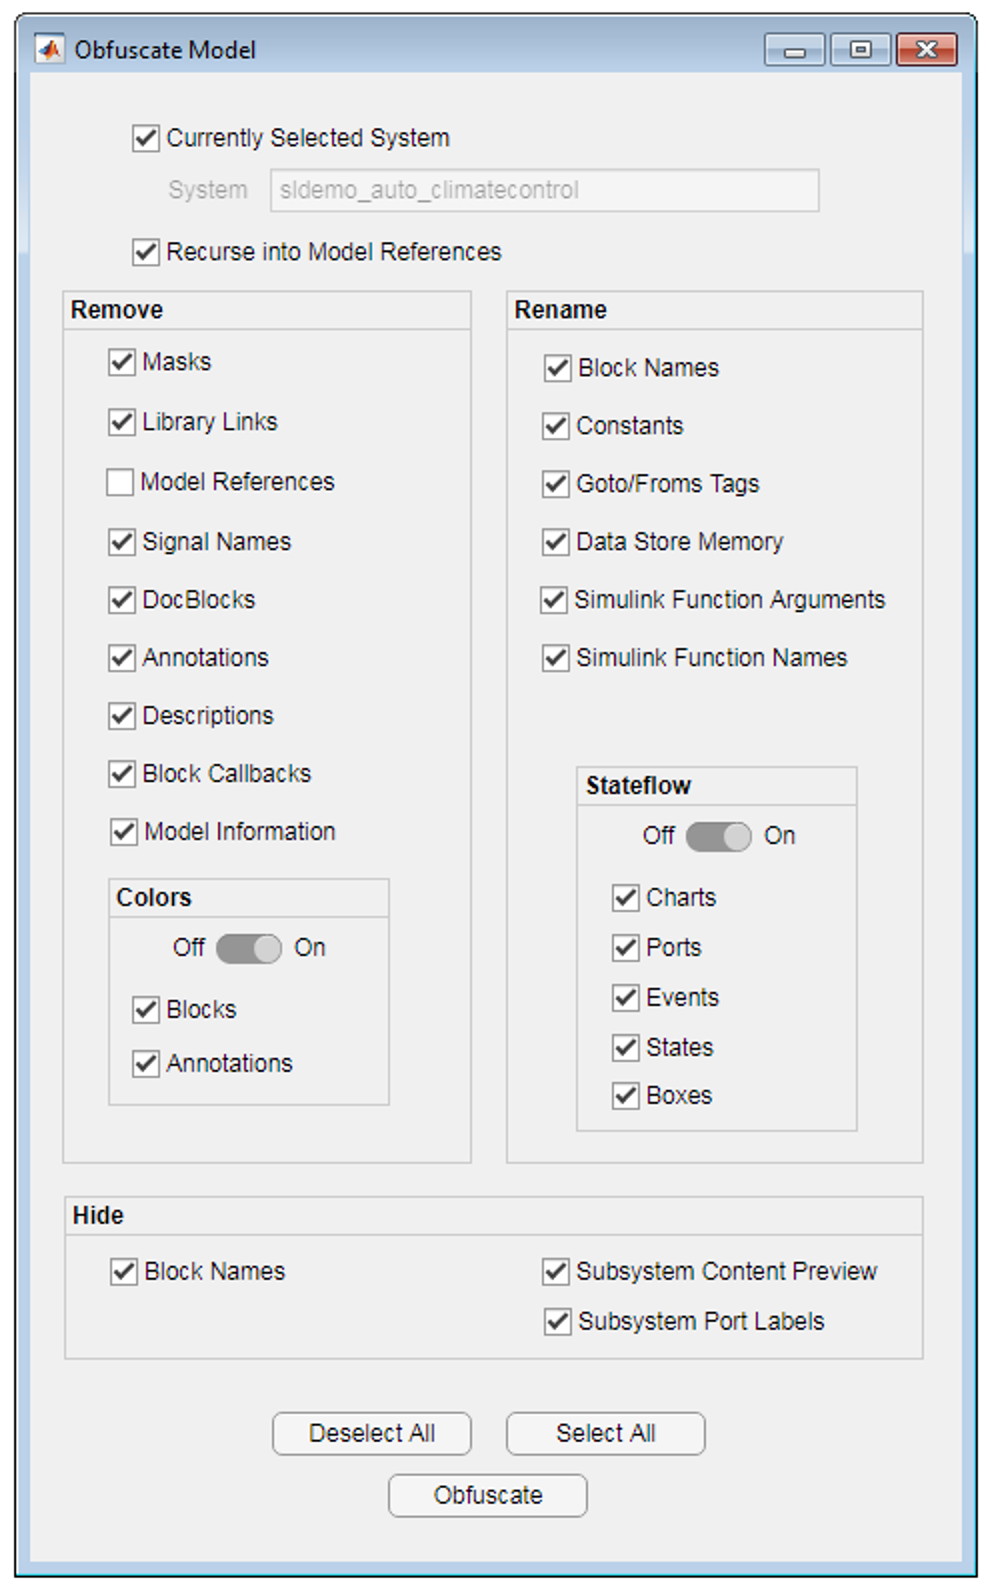
\includegraphics[width=0.7\textwidth]{../figs/GUI}
	\caption{The tool GUI.}
	\label{fig:contextMenu}
\end{figure}

%---------------------------------------
% What are the main uses of the tool?
%---------------------------------------
\newpage
\subsection{Functionality}
This section describes the tool functionality when being used from the GUI (Figure~\ref{fig:contextMenu}). Each section describes one of the groups of options in the GUI.

\subsubsection{Recurse into Model References}
This check-box will apply the removing (Section~\ref{lbl:remove}), renaming (Section~\ref{lbl:rename}), and hiding (Section~\ref{lbl:hide}) options inside of any referenced models.

\subsubsection{Remove}
\label{lbl:remove}
The options in the \emph{Remove} group will discard elements of the model.

\begin{itemize}
	\item Masks -- Block \href{https://www.mathworks.com/help/simulink/ug/block-masks.html}{masks} are commonly used to customize the block appearance of custom blocks. This option removes the masks of all blocks. 
	
	\item Library Links -- Library \href{https://www.mathworks.com/help/simulink/ug/creating-and-working-with-linked-blocks.html}{links} can be used in a model to reference blocks that reside in other libraries. This option removes (or ``breaks") all library links so that blocks are stored directly in the model instead of the library. This means that the model is no longer dependant on external libraries.
	
	\item Model References -- The use of a \href{https://www.mathworks.com/help/simulink/slref/model.html}{model} block introduces a reference to another model. This option resets all model reference blocks so that they no longer point to other models. \emph{Note: This may impact the model functionality.}
	
	\item Signal Names -- This option turns off \href{https://www.mathworks.com/help/simulink/ug/signal-label-propagation.html}{signal propagation}.
	
	\item DocBlocks -- A \docblock stores \href{https://www.mathworks.com/help/simulink/slref/docblock.html}{documentation} about the model. This options removes all \docblock{s}.
	
	\item Annotations -- This option deletes all text, area, or image \href{https://www.mathworks.com/help/simulink/ug/annotations.html}{annotations}.
	
	\item Descriptions -- This options removes the \param{description} information of \href{https://www.mathworks.com/help/simulink/ug/signal-basics.html#bs9gzwp}{lines}, \href{https://www.mathworks.com/help/simulink/ug/block-properties-dialog-box.html}{blocks}, and annotations. 
	
	\item Block Callbacks -- Blocks can have custom \href{https://www.mathworks.com/help/simulink/ug/block-callbacks.html}{callbacks}. This option removes all callbacks.
	
	\item Model Information -- A \Simulink model stores \href{https://www.mathworks.com/help/simulink/ug/managing-model-versions.html}{information} about itself, such as its creator's name and version number (Figure~\ref{fig:model_history}). This option resets this data.
	
\begin{figure}[htb]
	\centering
	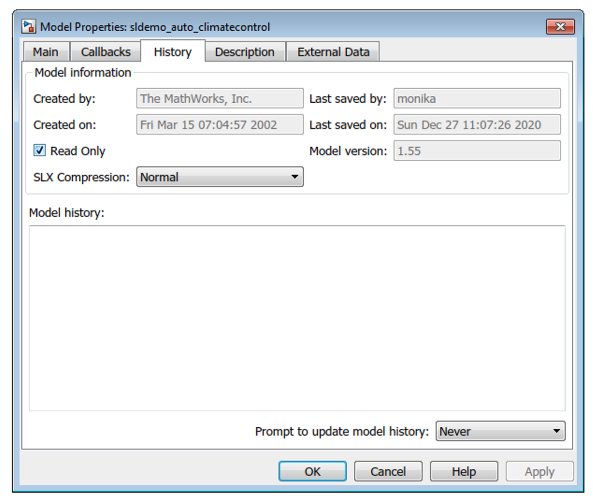
\includegraphics[width=.97\textwidth]{../figs/ModelHistory}
	\caption{Model Information.}
	\label{fig:model_history}
\end{figure}
	
	\item Colors -- These options remove the colours of blocks and annotations so that they revert to their default color.
\end{itemize}

\subsubsection{Rename}
\label{lbl:rename}
The options in the \emph{Rename} group will rename elements of the model to use generic names.

\begin{itemize}
	\item Block Names -- Each block in a model has a \param{name} that is typically displayed underneath the block. This option renames all block names to a generic name based on the block type. For example, an \inport block will be renamed to Inport1.
	
	\item Constants -- Each constant block has a \param{value} that is a number or a variable name. This option renames any values that are variable names to be generic (\eg Constant1). Numerical constants will remain. \emph{Note: You must manually change the definition of the data to match the new name. This tool does not currently rename data in the base workspace or data dictionaries.}
	
	\item Goto/From Tags -- A \goto block has a \param{goto tag} that matches it to its \from blocks. This option renames tags to generic names (\eg GotoFrom1) and renames any matching \from blocks as well.
	
	\item Data Store Memory -- A \DSM block has a \param{data store name}. This option renames all  \DSM blocks to be generic (\eg DataStore1) as well as all associated \DSR and \DSW blocks.
	
	\item Simulink Function Arguments -- A \simfunc can have inputs and outputs using \argin and \argout blocks. This option renames the \param{argument name} of \argin and \argout blocks to be generic (\eg u1 for an input, y1 for an output).

	\item Simulink Function Names -- The trigger within a \simfunc specifies the function's name. This option renames it to a generic name (\eg f1), and updates any corresponding \simfunccaller blocks to match.
	
	\item Stateflow -- These options rename the various named \href{https://www.mathworks.com/help/stateflow/ug/overview-of-stateflow-objects.html}{Stateflow elements} to have generic names. Currently inputs, outputs, events, boxes, and states are renamed.
\end{itemize}

\subsubsection{Hide}
\label{lbl:hide}
The options in the \emph{Hide} group will hide elements of the model from view.

\begin{itemize}
	\item Block Names -- This option hides the name of a block from view.
	
	\item Subsystem Content Preview -- This option turns off the \href{https://www.mathworks.com/help/simulink/ug/preview-content-of-hierarchical-items.html}{content preview} that is displayed in blocks such as subsystems.
	
	\item Subsystem Port Labels -- This option hides the port labels shown on blocks such as subsystems.

\end{itemize}

%---------------------------------------
% What else does the tool do?
%---------------------------------------
%\subsection{Errors and Warnings}
%Any errors or warnings during tool use will be visible in the \Matlab Command Window.

%%%%%%%%%%%%%%%%%%%%%%%%%%%%%%%%%%%%%%%%%%%%%%%%%%%%%%%%%%%%%%%%%%%
% Example
%%%%%%%%%%%%%%%%%%%%%%%%%%%%%%%%%%%%%%%%%%%%%%%%%%%%%%%%%%%%%%%%%%%
\section{Example}

Use the command \demoName in the \Simulink Command Window to open the example model, shown in Figure~\ref{fig:demo1}. To run the tool, run the command \cmd{ObfuscateModelGUI} from the Command Window, and then press the \cmd{Obfuscate} button. The resulting model is given in Figure~\ref{fig:demo2}. We can see that the colors, annotations, masks, names, port labels, and many other elements have been removed, renamed, or hidden in the model.

\begin{figure}[htb]
	\centering
	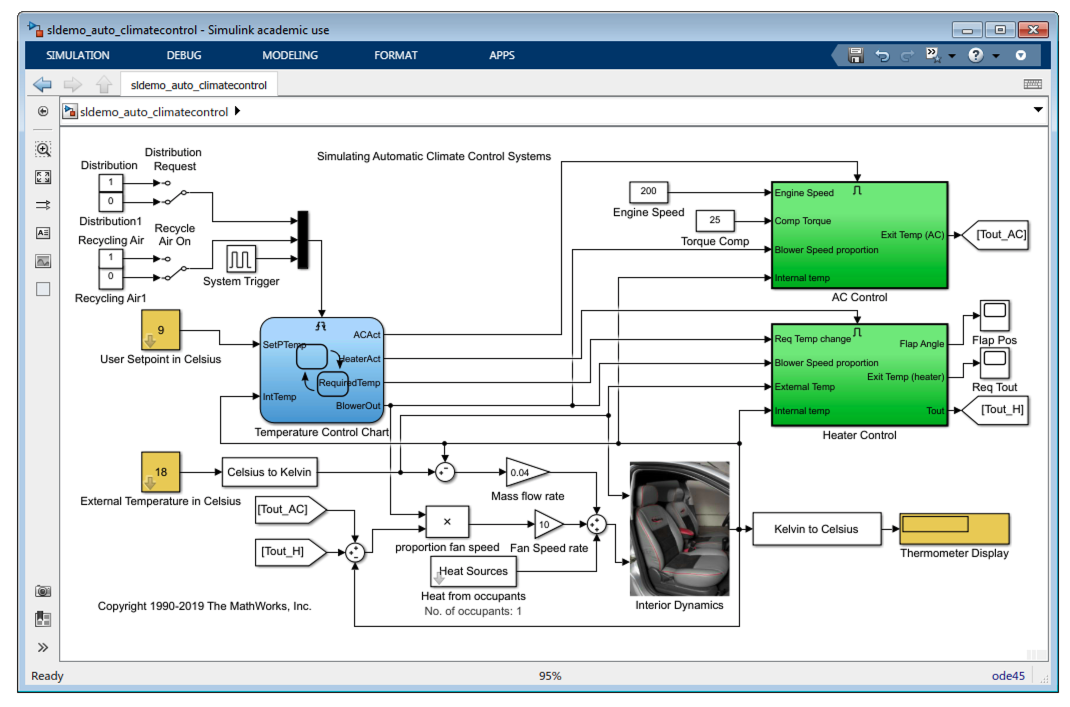
\includegraphics[width=.97\textwidth]{../figs/Demo1}
	\caption{Original demo model.}
	\label{fig:demo1}
\end{figure}

\begin{figure}[htb]
	\centering
	\makebox[\textwidth][c]{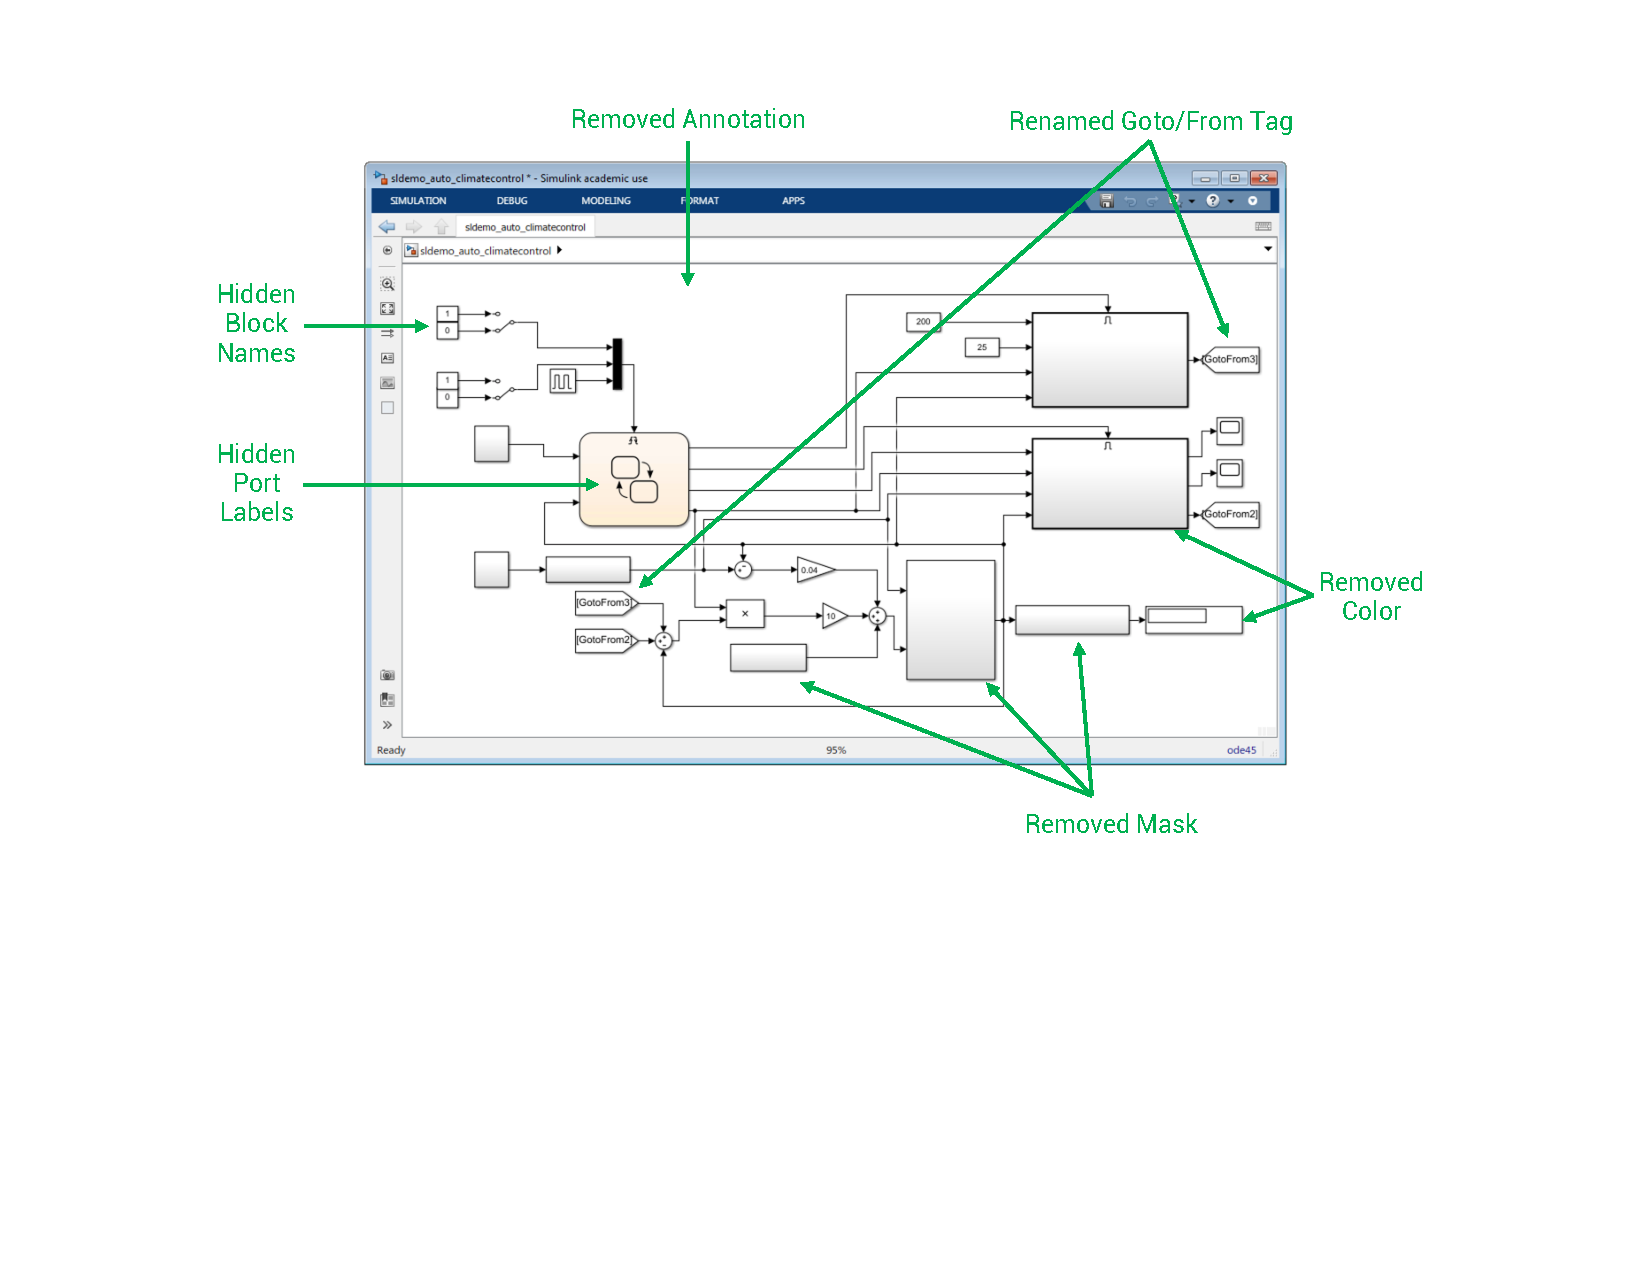
\includegraphics[width=1.25\textwidth]{../figs/Demo2_annotated}}
	\caption{Resulting model after obfuscation.}
	\label{fig:demo2}
\end{figure}

\end{document}